\section{JFileChooser}
\label{sec:JFileChooser}

Mithilfe des JFileChoosers wird es dem Benutzer ermöglicht, Dateien und Ordner auszuwählen. Dieser kann mit den verschiedensten Methoden angepasst werden. Dafür muss dieser jedoch bereits vorher initialisiert werden.

\begin{lstlisting}[language=JAVA]
JFileChooser chooser = new JFileChooser();
\end{lstlisting}
    
Nun kann man verschiedenste Einstellungen vornehmen. Sehr oft, wurde von uns ein so genannter FileNameExtensionFilter verwendet. Mit diesem ist es möglich. Dateien mit bestimmten Endungen herauszufiltern und nur diese anzeigen zu lassen.

Dies wurde zum Beispiel beim Suchen nach C-Compact Profilen verwendet!
\begin{lstlisting}[language=JAVA]
FileFilter filter = new FileNameExtensionFilter("CMM Profile",".cp");
chooser.setFileFilter(filter);
\end{lstlisting}



\subsection{Anzeigen einer Vorschau}
Bei der Implementierung des JFileChoosers, wurde oftmals ein Zusatz hinzugefügt, dem es den Nutzer ermöglicht eine Vorschau eines Bildes sowie den Nutzernamen zu haben.

\begin{figure}[h] 
  \centering
     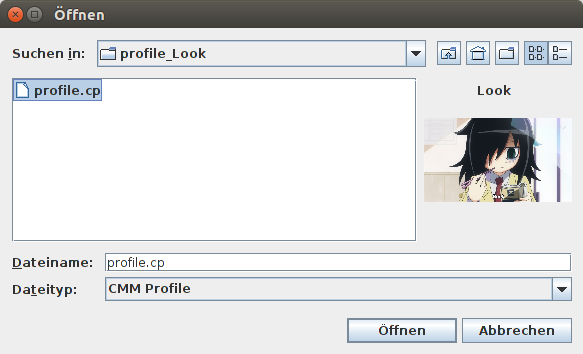
\includegraphics[width=0.9\textwidth]{./media/images/gui/launcher/launcher_finden.png}
  \caption{ Profilvorschau}
  \label{fig:Bild1}
\end{figure}

Die Vorschau wird in einer Klasse erstellt, welche ein JPanel erweitert und den PropertyChangeListener implementiert. Beim Anlegen des Konstruktors ist darauf zu achten das das Panel eine geeignete Größe zugewiesen bekommt.

Zuerst wird das PropertyChangeEvent abgerufen, welches beim Klicken auf eine Datei oder einen Ordner auftritt. Nun wird die Variable welche übergeben wurde, auf ein File gecastet. Somit kann nun abgefragt werden, ob es sich hierbei um den gewünschten Datentyp handelt. 
\begin{lstlisting}[language=JAVA]
	public void propertyChange(PropertyChangeEvent e) {
		String propertyName = e.getPropertyName();

		if (propertyName.equals(JFileChooser.SELECTED_FILE_CHANGED_PROPERTY)) {
			File selection = (File) e.getNewValue();
			...
			}
\end{lstlisting}

Nun muss das Bild nur mehr geladen und skaliert werden, und kann mithilfe der paintComponent Methode in den JFileChooser eingeschleust werden.

Nun kann die neue Klasse eingebunden werden. Dies geschieht indem man mehrere vorgegebene Klassen verwendet. Hierbei ist setAccessory für extra Componenten, und PropertyChangeListener für Events die im JFileChooser ausgeführt werden zuständig.
\begin{lstlisting}[language=JAVA]
		ProfilePreviewPanel preview = new ProfilePreviewPanel();
		chooser.setAccessory(preview);
		chooser.addPropertyChangeListener(preview);
\end{lstlisting}